The following section illustrates how the sequences are encoded for perceptual test and how we choose our selection of bitrate targets to limit the test duration. 

\begin{figure}[bht!]
	\centering
	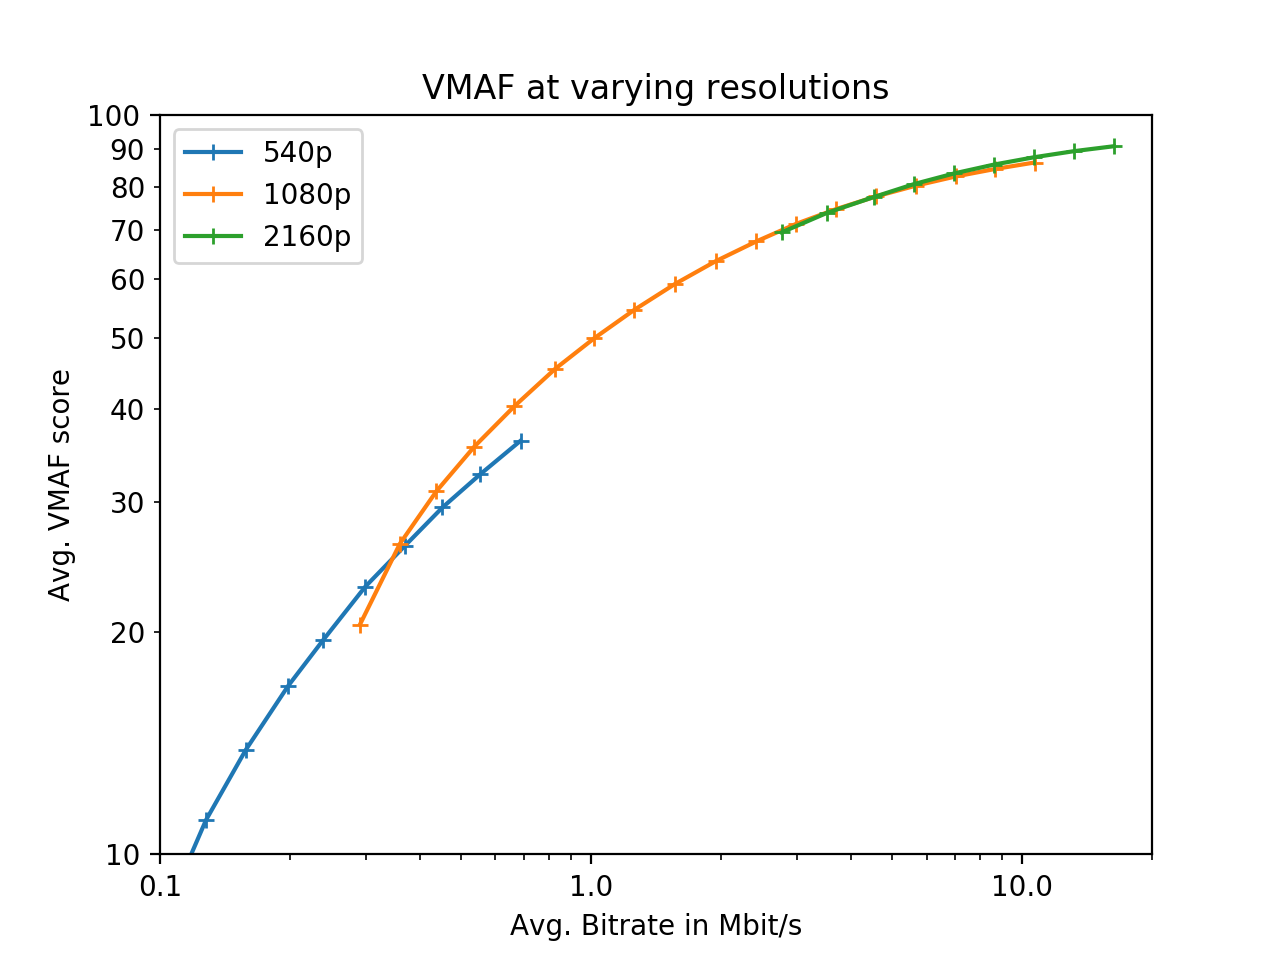
\includegraphics[width=3.5in]{vmaf_bitrates}
	\caption{Average VMAF scores for 25 different bitrates at 3 resolutions. The encoded bitrates and the VMAF scores are averaged between the 6 sequences and form the abscissa (Log) and ordinate respectively.}
	\label{fig:vmaf:bitrates}
\end{figure}

\subsubsection{Encoding Presets}
Two different presets are used for the sequence encodings, a "na\"{\i}ve" (P.1) and an "expert" preset (P.2). The "na\"{\i}ve" preset is a simple CBR encoding, whereas the "expert" preset is a 2-pass encoding with a Q-CTRL pass followed by a B-CTRL pass.  Every sequence is encoded with both presets at 3 resolutions (540p, 1080p, 2160p) and 3 bitrates for each resolution. The resulting VMAF-scores for the encoded sequences can be seen in Figure \ref{fig:vmaf:encoded}. The following section explains our method for the bitrate selection.

\subsubsection{Selection of Bitrates}
Video Multi-Method Assessment Fusion (VMAF) is a full reference metric for estimating human perception of video quality \cite{lin2013:mmf}. We use it because it provides a better estimate of subjective quality than single metrics like SSIM or VIF.

To estimate relevant HEVC bitrates for our source content we sample the VMAF scores at 25 bitrates on a logarithmic scale for our 3 different resolutions (540p, 1080p, 2160p). The reference sequences are resampled to a fixed 50 frames per seconds to avoid frame rate differences, while the distorted sequences are downsampled, encoded with CBR rate control and upsampled to UHD-1 again using lanczos resampling. Both presets use 4:2:0 chroma subsampling to be close to the typical use-case of webvideo. The resulting VMAF scores exhibit an overlap between different resolutions and the final encoding bitrates are chosen near those intersections. Figure \ref{fig:vmaf:bitrates} shows the sampled scores with the target rates in the background. We choose the target bitrates at least 2 bitrate-samples away from an intersection with the next quality, except for the lower 1080p-bound where it is not possible to lower the bitrate any further due to encoder restrictions. This should ensure a relevant sampling of the MOS-bitrate space for the subjective test.

\begin{figure}[bht!]
	\centering
	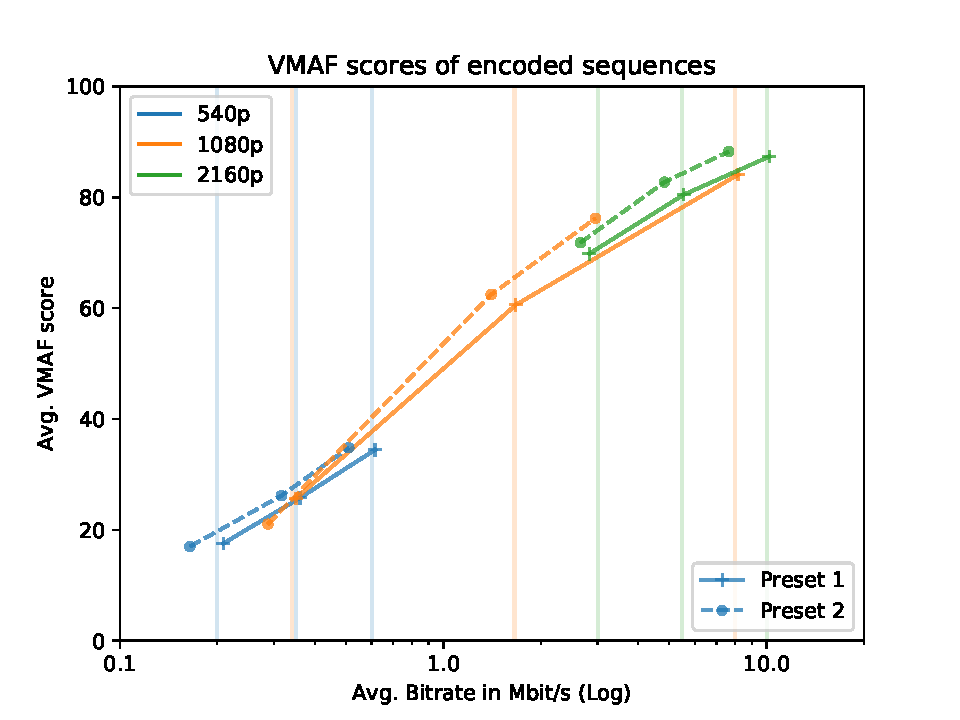
\includegraphics[width=3.5in]{vmaf_final}
	\caption{Average VMAF scores of encoded videos for both presets. The encoded bitrates and the VMAF scores are averaged between the 6 sequences for each preset and form the abscissa (Log) and ordinate respectively.}
	\label{fig:vmaf:encoded}
\end{figure}

The average VMAF scores of the two presets at the chosen bitrates can be seen in Figure \ref{fig:vmaf:encoded}. The target bitrates can again be seen in the background. The scores of the "expert" preset are consistently higher than the ones for the "na\"{\i}ve" preset at matching bitrates. Furthermore the "expert" preset saves bitrate by resorting to an acceptable level of quality, while the "na\"{\i}ve" presets bitrates are very close to the targets.


\begin{figure}[bht!]
	\centering
	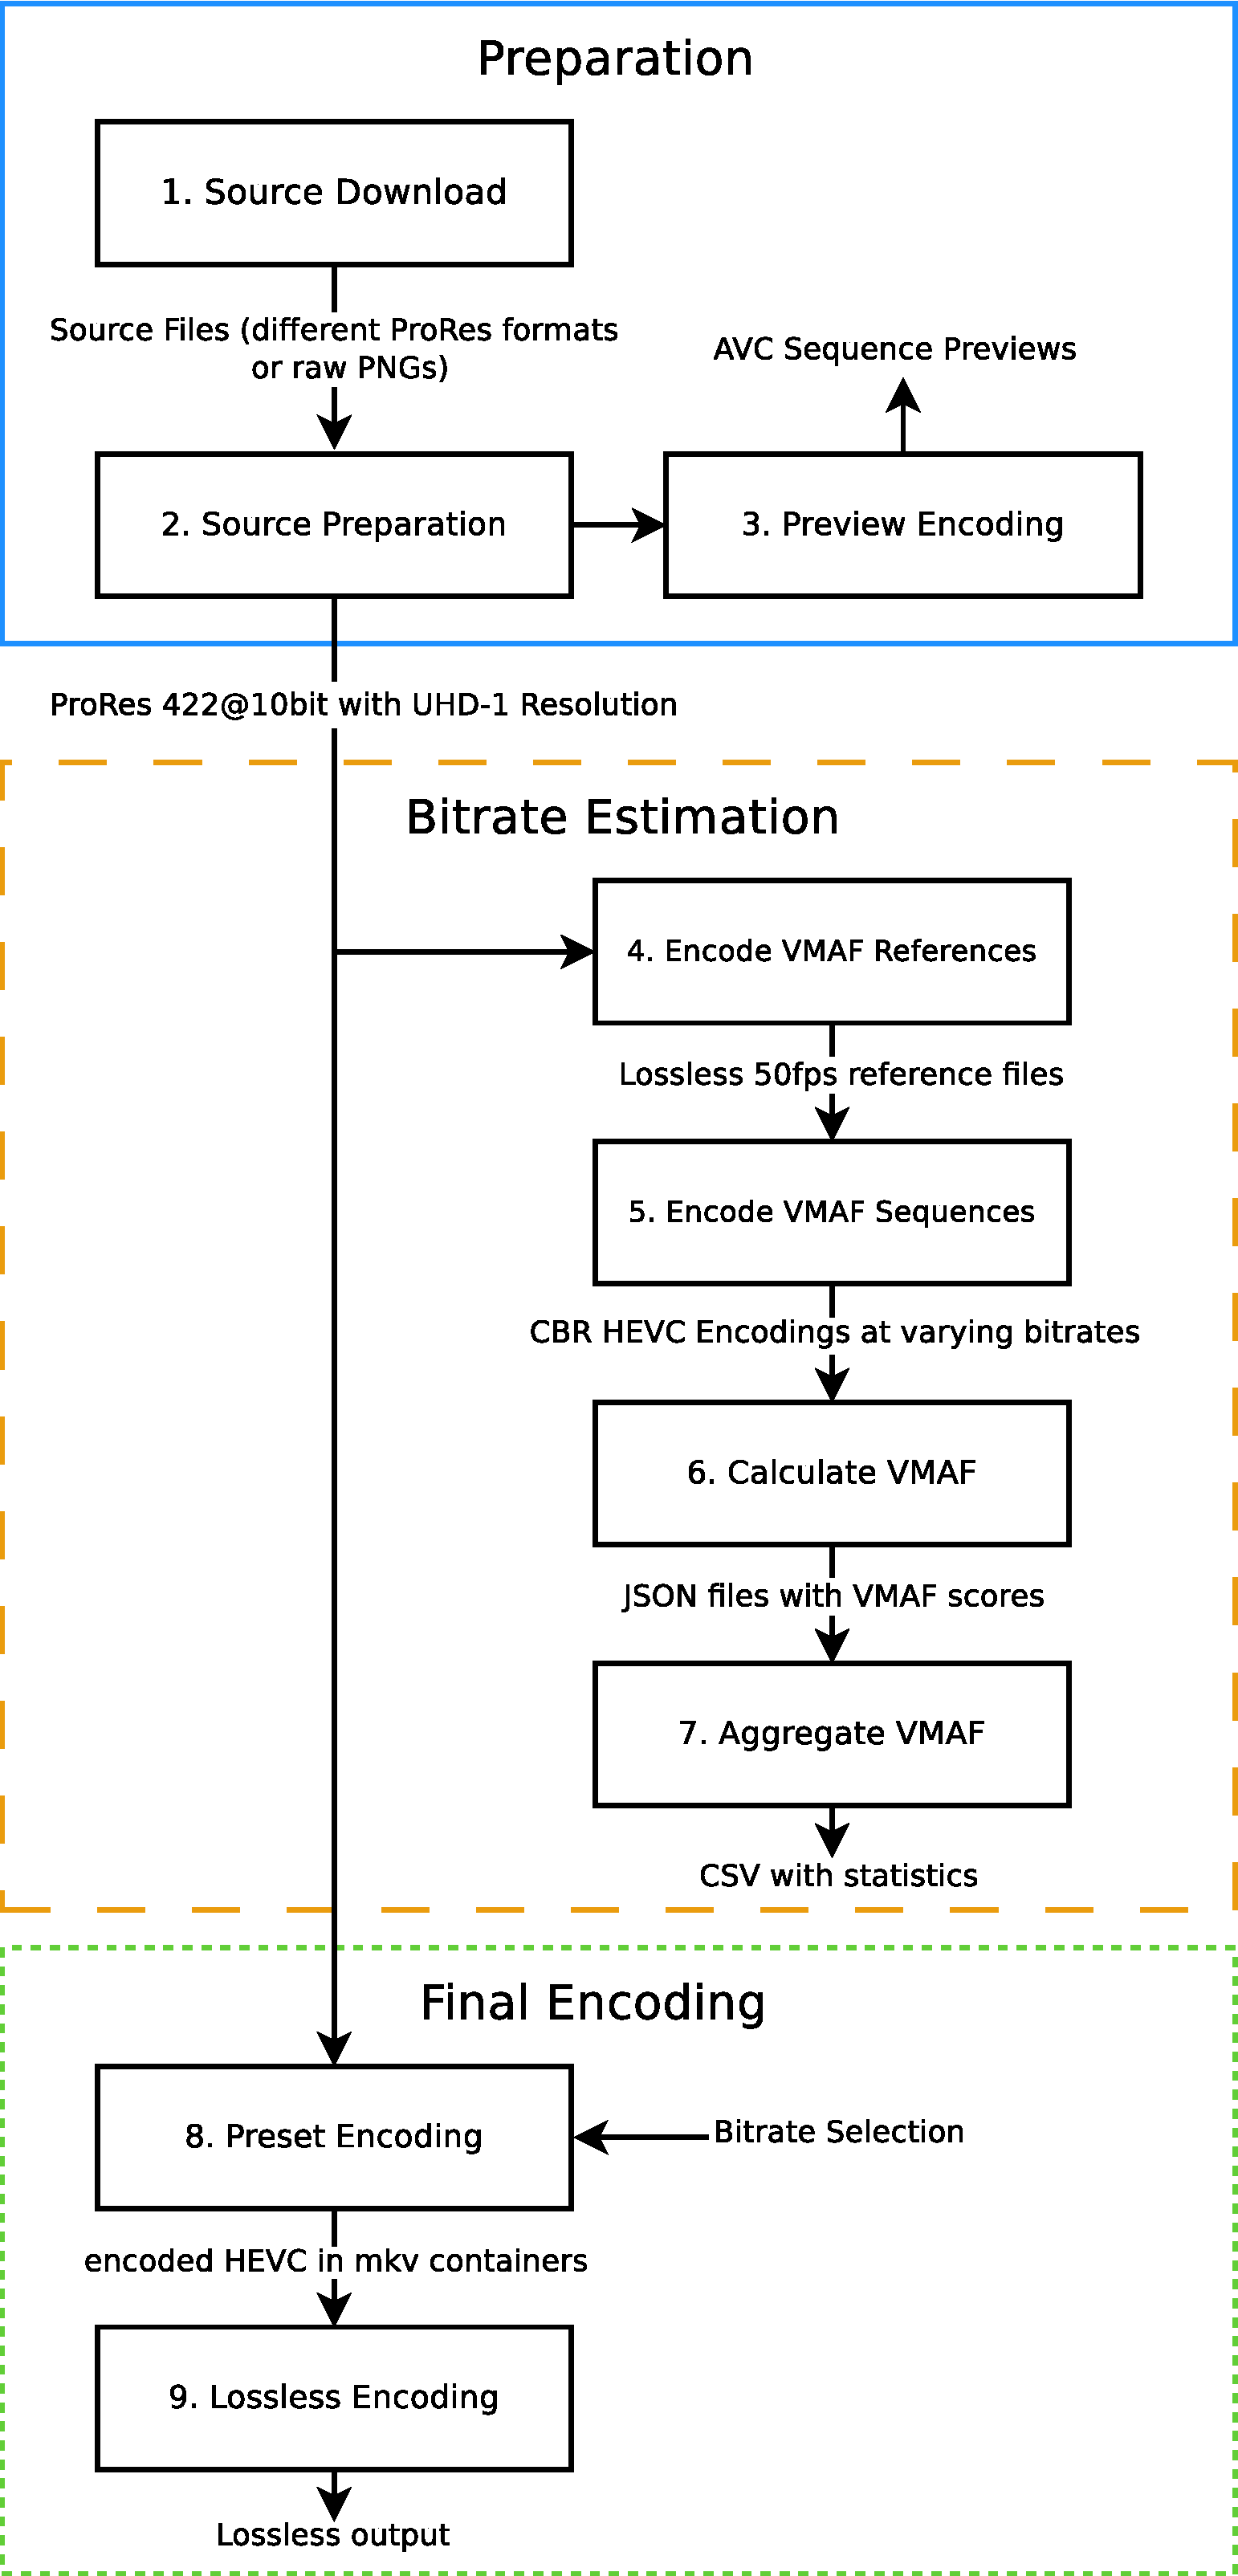
\includegraphics[width=2.5in]{automation}
	\caption{Automated processing and encoding workflow.}
	\label{fig:automation}
\end{figure}

\subsubsection{Encoding Automation}
We automate the whole process for downloading, preprocessing and encoding the source videos using pydoit \cite{web:pydoit}. This speeds up the turnaround time for changed parameters or sequences and also ensures that the encoded material can later be reproduced.

The whole process is illustrated in Figure \ref{fig:automation} and starts with the source preparation (A). After download of the sequences (1) they are cut to 10 seconds length and saved as ProRes HQ with UHD-1 resolution (2). Additionally, MPEG-4 AVC previews are generated at a lower resolution of 1440p to allow review of the sequences on slower devices.

After the initial processing the bitrate estimation is performed (B) using the VMAF metric \cite{lin2013:mmf}. The videos are brought to the same frame rate of 50fps (4) and encoded with CBR at 25 different bitrates (5). The average VMAF score of each video is analyzed with the VMAF Development Kit (VDK) \cite{web:vdk} and saved as a json file (6). All of the scores are then aggregated into a single CSV for plotting and further analysis (7).

The main encoding takes place last (C). Final encoding requires bitrate selection, which is performed manually. The sequences are encoded with the presets first (8) and then transcoded to a lossless format (ffvhuff) to allow for fast and consistent playback as well as archiving the video material.


